%!TEX root = Tesi__Simone_Mariotti.tex
\chapter{Componenti del robot}
\section{Hardware}
\subsection{UDOO Quad}
UDOO è un progetto tutto italiano di una piattaforma hardware destinata alla generazione dei ``makers'', cioè quelle persone che vogliono realizzare i proprie progetti bcon le tecnologia a basso costo ad oggi disponibili. La scheda ha visto la luce dopo una soprendente campagna di crowdfunding\footnote{dall'inglese crowd, folla e funding, finanziamento. In italiano finanziamento collettivo.} terminata l'8 Giugno 2013 con 4172 donazioni per un totale di \$641.612 a fronte di \$27.000 richiesti per iniziare la produzione. Per permettere l'utilizzo di librerie e applicazioni computazionalmente pesanti come openCV, PureData e altre UDOO monta un processore ARM Freescale i.MX6 Cortex-A9 Quad core 1GHz che supporta sia Android che Linux. Il tutto è completato da una GPU Vivante, 1GB di RAM DDR3, numerose porte di I/O come SATA, microfono, audio out, Ethernet, HDMI, USB, connettore per display LVDS con touch screen, connettore CSI per camera esterna e connettività bluetooth e Wi-Fi. La periferica di ``boot'' è una microSD il che permette un rapido passaggio da Linux a Android e viceversa. Quello che però rende veramente unica questa piattaforma, e che ne ha fatto la nostra scelta per questo progetto di tesi, è la presenza di un Arduino DUE completamente integrato nella stessa board. 
E' presente una CPU Atmel SAM3X8E ARM Cortex-M3 \footnote{la stessa di cui dispone l'Arduino DUE} e 76 GPIO\footnote{General Purpose Input/Output}, di cui 62 digitali e 14 digitali/analogici, disposti per essere perfettamente compatibili con la piedinatura dell'Arduino DUE e dell'Arduino UNO Rev.3. \\
La presenza di un Arduino DUE all'interno della board rende UDOO una scheda di prototipazione a tutti gli effetti e apre nuovi interessanti scenari e possibilità unendo la versatilità e semplicità di Arduino, la potenza di calcolo del Freescale i.MX6 e le numerose periferiche disponibili per Linux o Android.\\
Essendo una piattaforma open-source è possibile accedere alla shell del sistema operativo come root tramite la porta seriale integrata e modificare a piacimento la configurazione del sistema operativo. Arduino è collegato al Freescale i.MX6 tramite un bus interno e quindi viene rilevato come una normale periferica USB da Linux; su Android la comunicazione tra i due dispositivi avviene sullo stesso bus ma usa lo standard USB OTG\footnote{On-The-Go è una specifica che permettere di agire come host ad un qualsiasi  dispositivo (tipicamente smartphone e table). A differenza dell'USB classico l'OTG è driver-less, cioè non necessita l'installazione di driver specifici per ogni dispositivo}


\begin{figure}[ht] \center
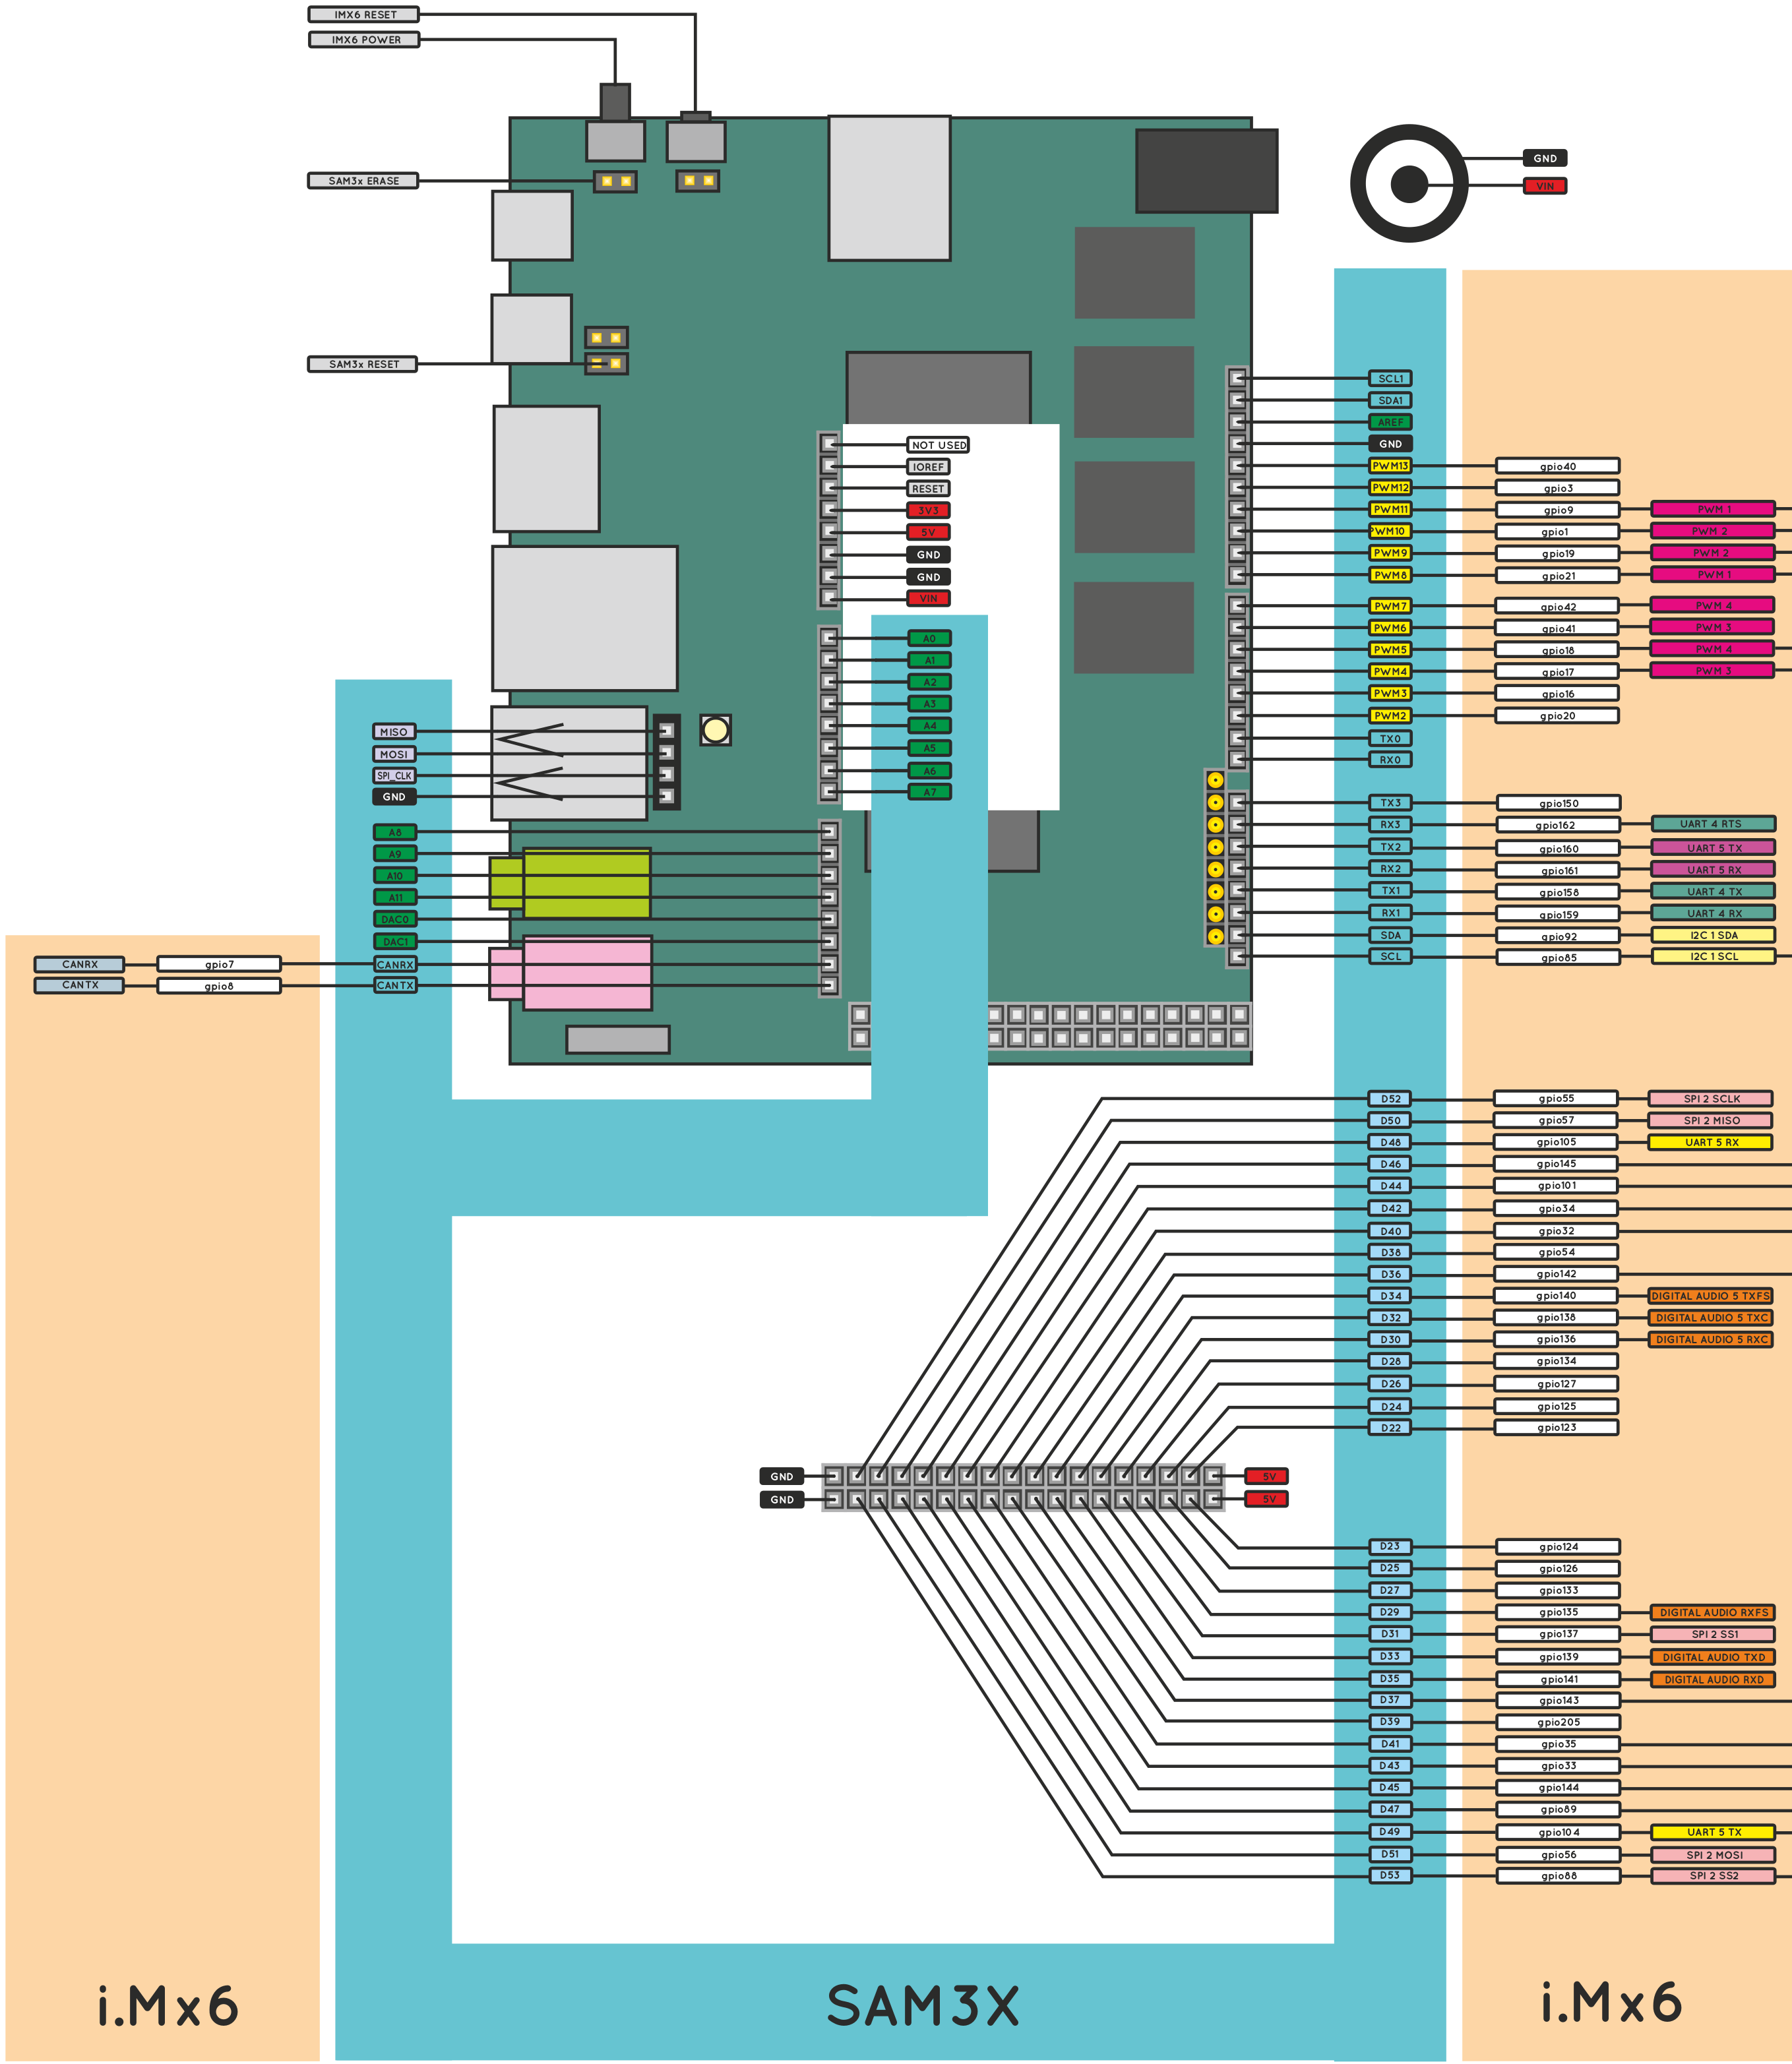
\includegraphics[width=\textwidth]{immagini/udoo_pinout.png}
\caption{Schema piedinatura UDOO} 
\end{figure}
\subsection {Tank Kit}
\subsection {Sensori}

\section{Software}
\subsection {OpenCV}
\subsection {ADK}
\subsection {ADK Toolkit}
